\chapter{METODE PENELITIAN}

\section{Deskripsi Data}
Dataset yang digunakan adalah \textit{Medical Sound Classification Challenge} yang diselenggarakan oleh Himanshu Kaushik pada platform Kaggle\cite{airs-ai-in-respiratory-sounds}. Dataset ini memiliki 882 jumlah data yang terdiri dari tiga jenis data untuk setiap individu yaitu audio batuk, vowel dan fitur riwayat pasien. Data diidentifikasi menggunakan candidateID yang ditetapkan untuk setiap orang. File suara dan embedding terdapat di folder candidateID yang diberikan. Dataset terbagi menjadi dua jenis yaitu 544 untuk data latih dan 338 untuk data uji yang belum memiliki label. Label penyakit terdiri dari 3 kelas yaitu asma, COPD dan pasien sehat.
\begin{figure}[H]
    \centering
    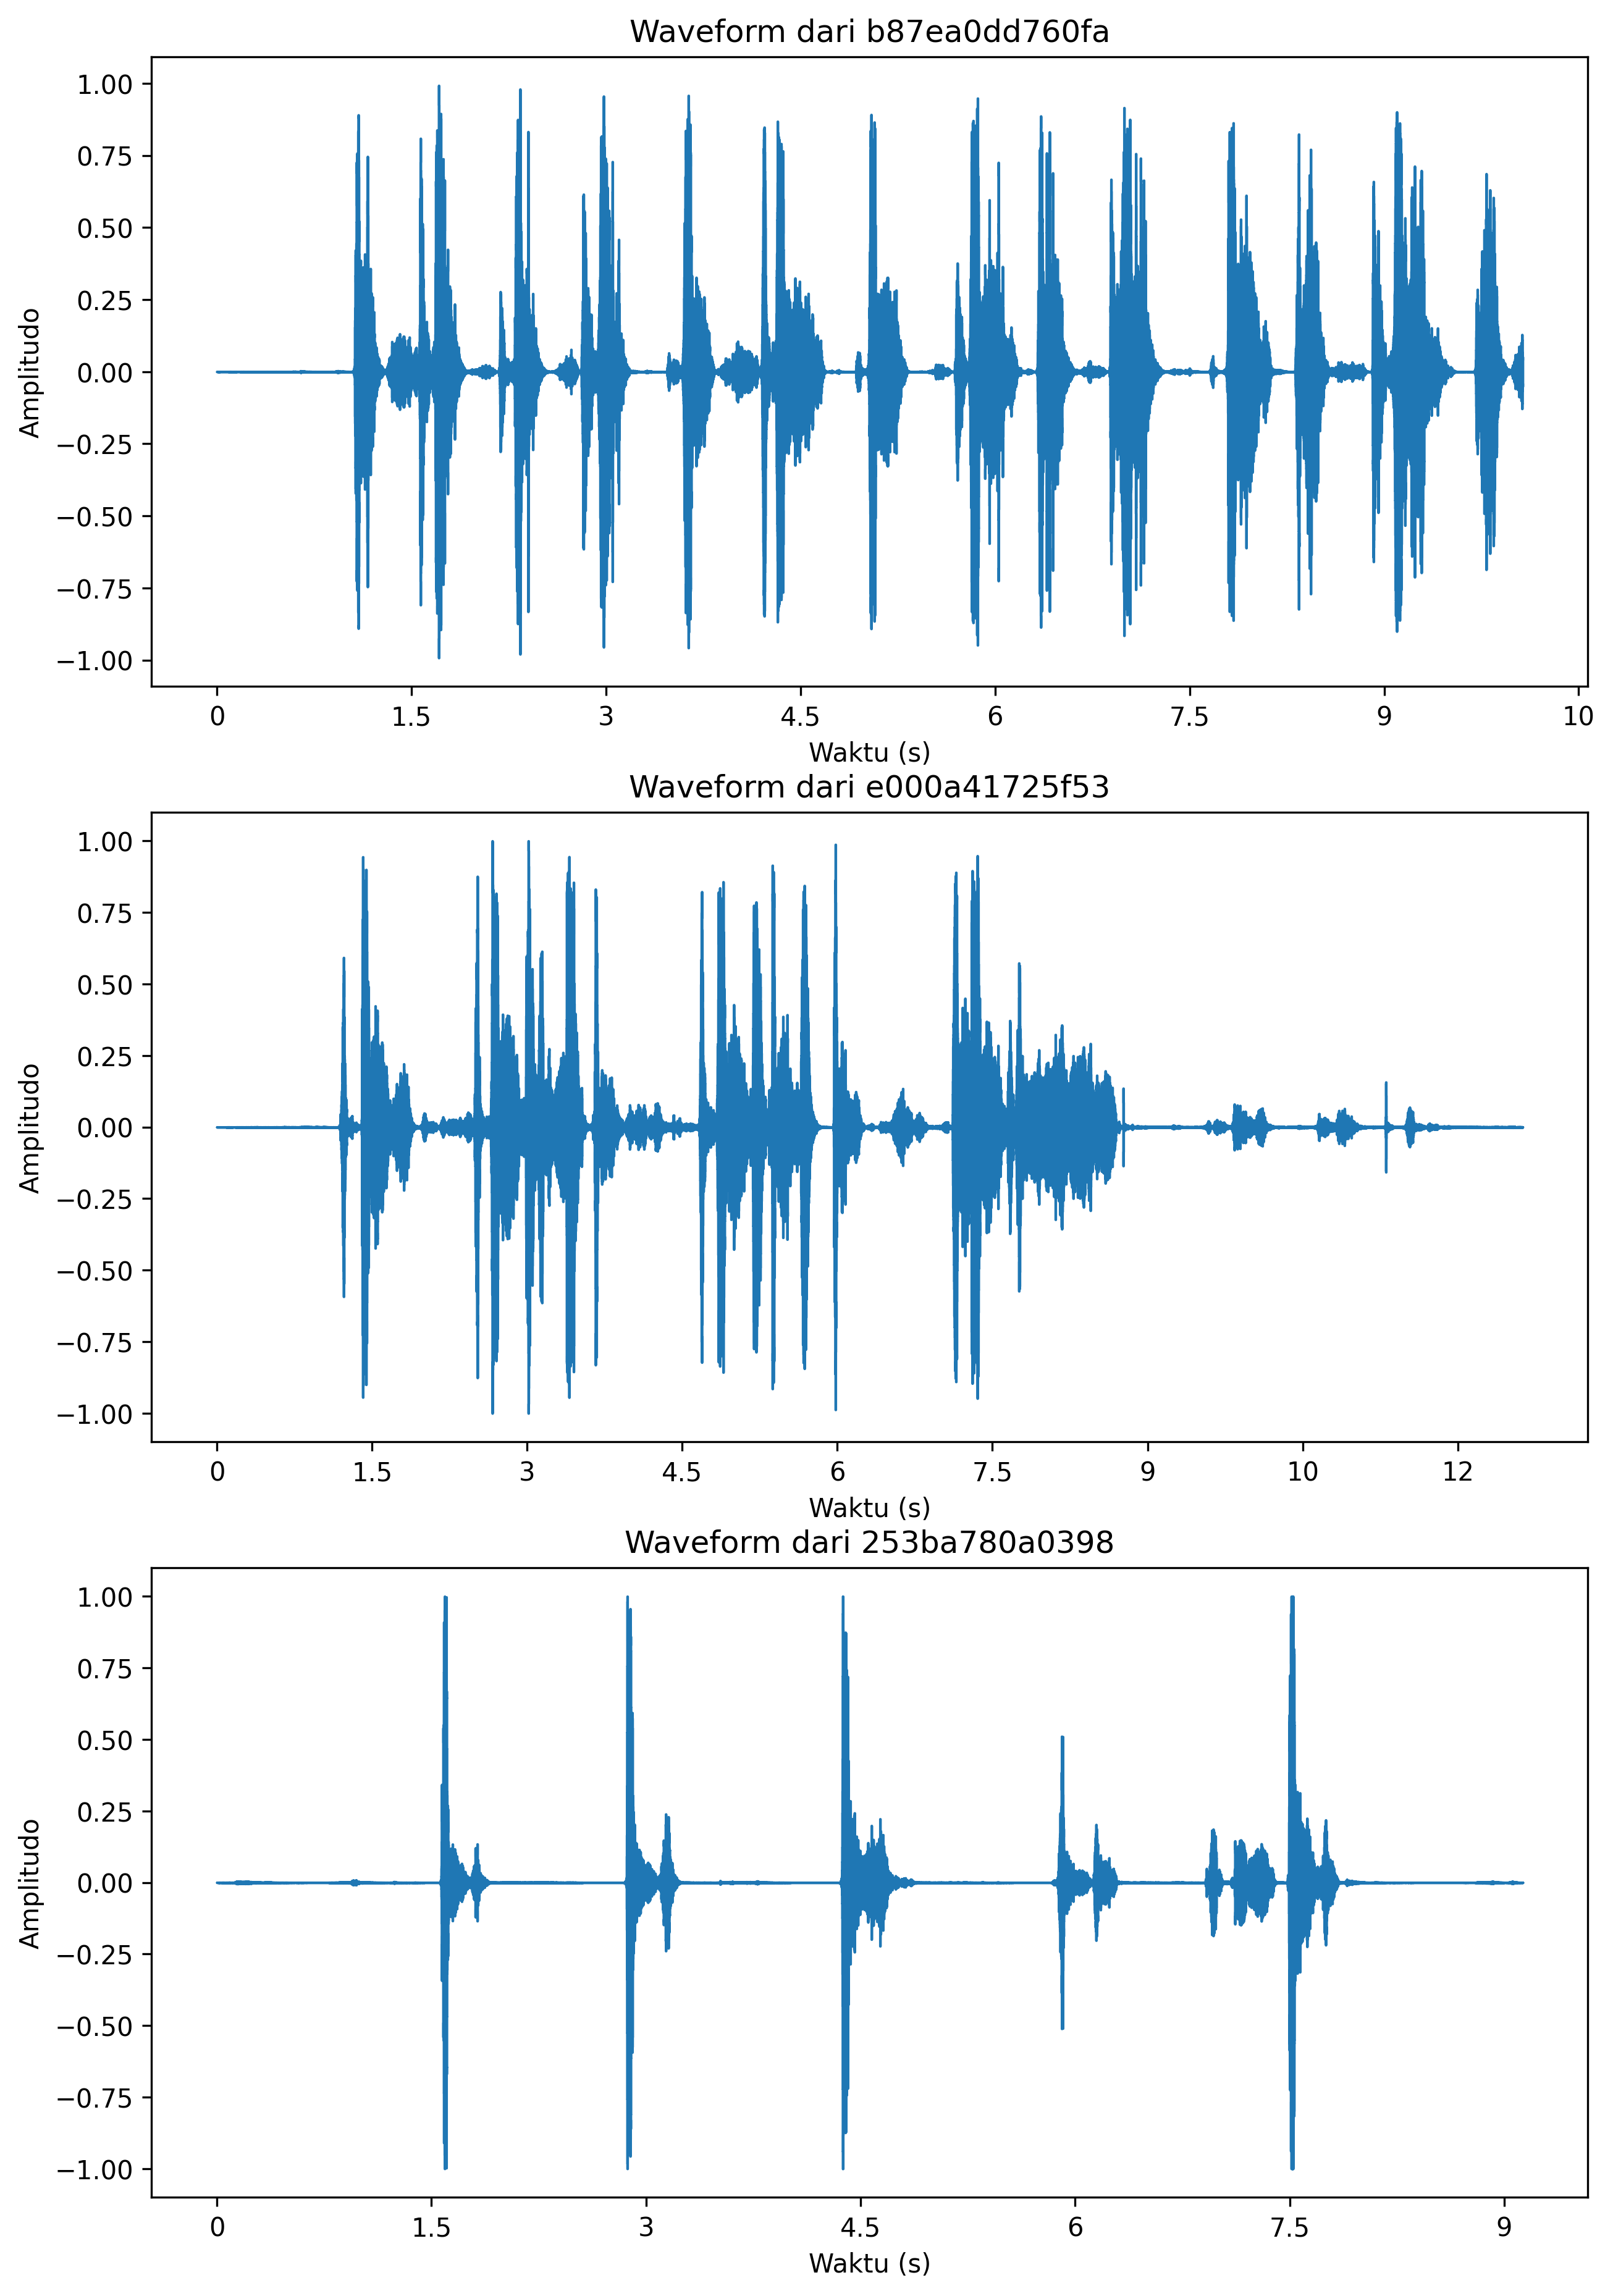
\includegraphics[width=0.7\linewidth]{gambar/waveforms.png}
    \caption{Visualisasi gelombang suara tiap kelas}
    \label{fig:waveform}
\end{figure}

\begin{landscape}
\begin{longtable}{p{3cm}lcccccccccc}
\caption{Tabel riwayat pasien}\\
\hline
\textbf{candidateID} & \textbf{age} & \textbf{gender} & \textbf{tbContact} & \textbf{wheezing} & \textbf{phlegmCough} & \textbf{familyAsthma} & \textbf{feverHistory} & \textbf{coldPresent} & \textbf{packYears} & \textbf{disease} \\ \hline
%\endfirsthead

%\multicolumn{4}{l}{\bfseries \tablename\ \thetable{} -- Lanjutan dari halaman sebelumnya}\\
% \begin{center}
% % {{\bfseries \tablename\ \thetable{} -- Lanjutan dari halaman sebelumnya}} \\
% \end{center}
%\hline
%\textbf{candidateID} & \textbf{age} & \textbf{gender} & \textbf{tbContact} & \textbf{wheezing} & \textbf{phlegmCough} & \textbf{familyAsthma} & \textbf{feverHistory} & \textbf{coldPresent} & \textbf{packYears} & \textbf{disease} \\ \hline

%\endhead

%\hline
%\endfoot

%\endlastfoot

2bbd6c5ecf1ce & 55 & 1 & 0.0 & 0.0 & 0.0 & 1.0 & 0.0 & 0.0 & 0 & 1 \\
75fa6e335b5ca & 65 & 0 & 0.0 & 1.0 & 0.0 & 0.0 & 0.0 & 1.0 & 560 & 2 \\
7dc99cfcb5aa & 43 & 0 & 0.0 & 1.0 & 0.0 & 0.0 & 0.0 & 0.0 & 0 & 1 \\
59cf4a7821471 & 74 & 0 & 0.0 & 1.0 & 0.0 & 0.0 & 0.0 & 0.0 & 800 & 2 \\
59f9fe56c2f12 & 28 & 0 & 0.0 & 0.0 & 1.0 & 0.0 & 0.0 & 0.0 & 0 & 0 \\
caee891a86d8d & 56 & 1 & 0.0 & 1.0 & 0.0 & 0.0 & 0.0 & 0.0 & 0 & 1 \\
5b8578b39385f & 31 & 0 & 0.0 & 0.0 & 1.0 & 0.0 & 0.0 & 0.0 & 0 & 0 \\
f3e7d50ce7288 & 35 & 0 & 0.0 & 1.0 & 1.0 & 0.0 & 0.0 & 0.0 & 0 & 1 \\
ad5fa122d4efb & 56 & 1 & 0.0 & 0.0 & 0.0 & 1.0 & 0.0 & 0.0 & 0 & 0 \\
14b58d18c66c7 & 57 & 0 & 0.0 & 1.0 & 1.0 & 0.0 & 0.0 & 0.0 & 0 & 0 \\
7959121db060d & 48 & 0 & 0.0 & 1.0 & 0.0 & 0.0 & 0.0 & 0.0 & 0 & 1 \\
77aa6a34f6da1 & 21 & 0 & 0.0 & 0.0 & 1.0 & 1.0 & 0.0 & 0.0 & 0 & 1 \\
069276518f6f & 25 & 1 & 0.0 & 0.0 & 0.0 & 1.0 & 0.0 & 0.0 & 0 & 2 \\
3d71862ec1801 & 48 & 1 & 0.0 & 0.0 & 1.0 & 1.0 & 0.0 & 0.0 & 0 & 1 \\
1868d92d2db4 & 20 & 0 & 0.0 & 0.0 & 0.0 & 1.0 & 0.0 & 1.0 & 360 & 2 \\
fbf8398bd0136 & 70 & 0 & 0.0 & 0.0 & 1.0 & 0.0 & 0.0 & 0.0 & 0 & 1 \\
0343c366074ec & 25 & 0 & 0.0 & 1.0 & 1.0 & 0.0 & 0.0 & 0.0 & 0 & 1 \\ 
\dots & \dots & \dots & \dots & \dots & \dots & \dots & \dots & \dots & \dots & \dots \\ 
e17cb00bd9677 & 66 & 0 & 0.0 & 0.0 & 1.0 & 0.0 & 0.0 & 1.0 & 0 & 2 \\
\hline
\label{table:riwayat_pasien}
\end{longtable}
\end{landscape}

\section{Rancangan Penelitian}
\begin{figure}[H]
    \centering
    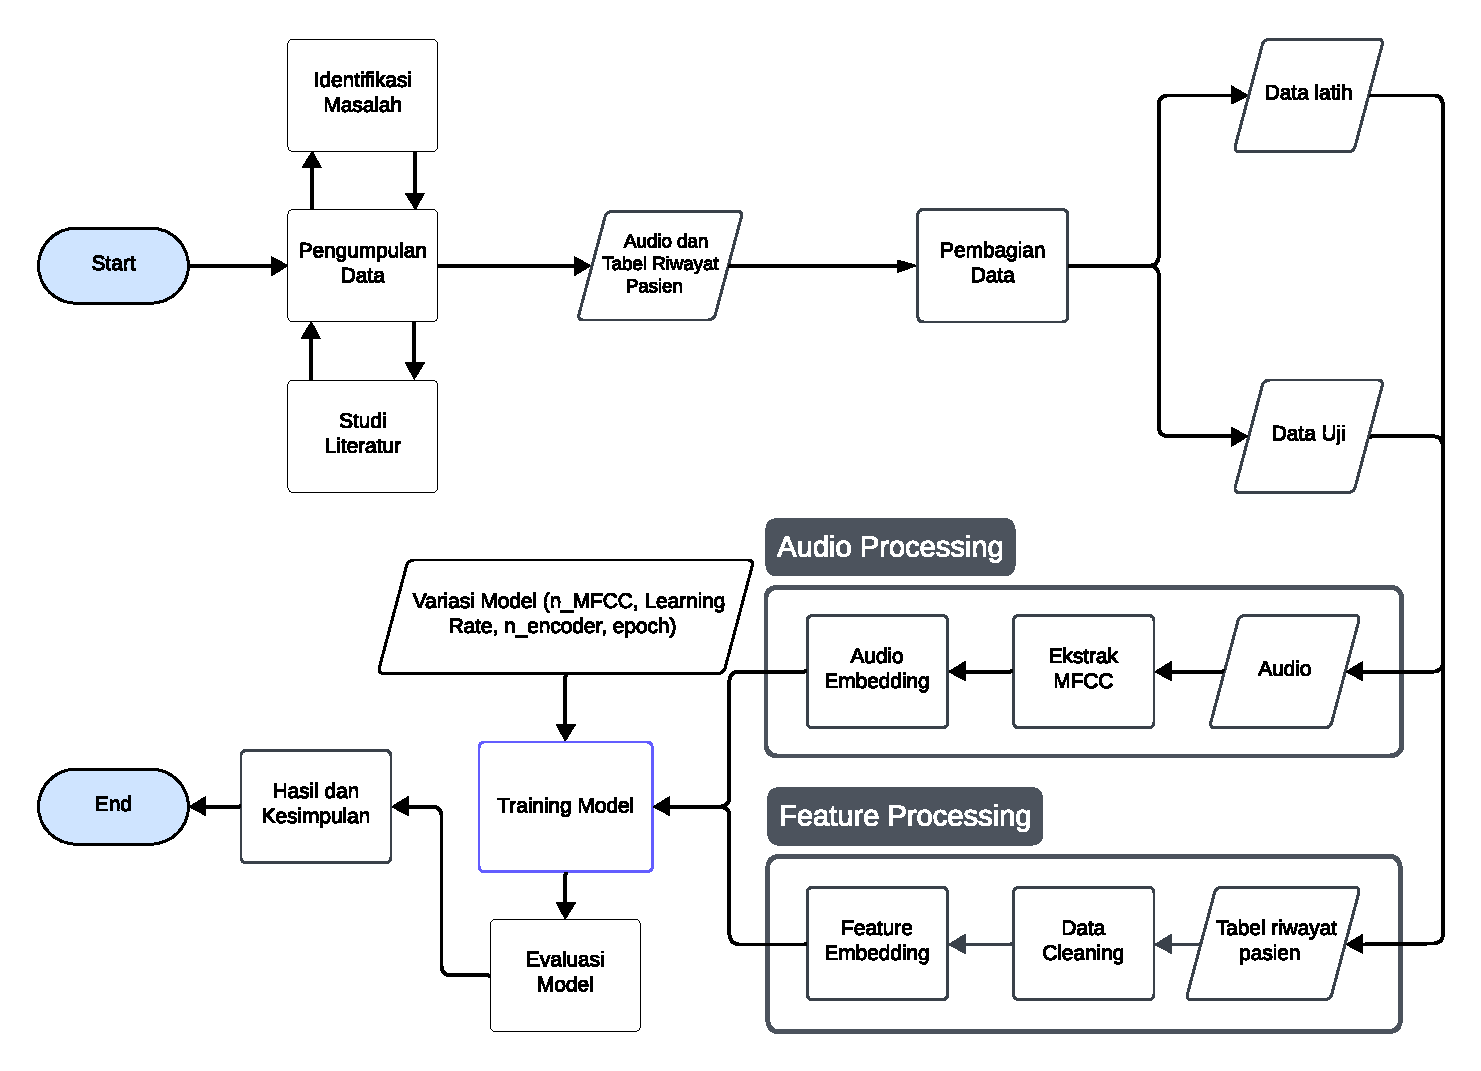
\includegraphics[width=1\linewidth]{gambar/Flowchart Rancangan Penelitian.pdf}
    \caption{\textit{Flowchart} rancangan penelitian}
    \label{fig:flowchart}
\end{figure}

    \subsection{Pengumpulan Data}
    Data diunduh ke dalam \textit{notebook} menggunakan kaggle-api dengan fungsi yang telah disediakan di laman kompetisi. File unduhan berupa .zip yang harus diekstrak terlebih dahulu.

    \subsection{Pembagian Data}
    Data dibagi menjadi data latih dan data uji dengan perbandingan 80\% untuk data latih dan 20\% untuk data uji. Digunakan parameter random state agar proses pembagian data bisa direproduksi ulang. Dilakukan \textit{stratified sampling} berdasarkan kolom target yaitu \textit{disease} untuk memastikan distribusi kelas tetap sama di kedua set.

    \subsection{Pemrosesan Suara}
    Data suara yang digunakan pada penelitian ini berupa suara batuk \textit{cough.wav} pasien yang berisi minimal 3 kali batuk, dengan durasi rekaman maksimal 15 detik. Dilakukan ekstraksi fitur menggunakan \textit{Mel frequency Capstral Coefficients} (MFCC), yaitu dengan cara memfilter secara logaritmik pada frekuensi di atas 1000 Hz dan secara linier pada frekuensi di bawah 1000 Hz. MFCC dapat meningkatkan sensitivitas pada suara dengan frekuensi rendah dan sebaliknya, pada suara dengan frekuensi tinggi MFCC dapat mengurangi sensitivitas dalam menangkap suara \cite{10593181}.
    \begin{algorithm}[H]
    \caption{Ekstraksi MFCC}
    \begin{algorithmic}[1]
    
    \Function{ExtractMFCC}{$file\_path, n\_mfcc, target\_length$}
        \State Load audio file and sampling rate: $(audio, sr) \gets \Call{Load}{file\_path}$
        \State Compute MFCC: $mfcc \gets \Call{ComputeMFCC}{audio, sr, n\_mfcc}$
        \State Transpose $mfcc$: $mfcc \gets mfcc^T$
        \If{$\text{length}(mfcc) > target\_length$}
            \State Trim $mfcc$ to $target\_length$
        \ElsIf{$\text{length}(mfcc) < target\_length$}
            \State Pad $mfcc$ with zeros
        \EndIf
        \State \Return $mfcc$
    \EndFunction
    
    \end{algorithmic}
    \label{algo:audio_process}
    \end{algorithm}

    \subsection{Pemrosesan Data Tabel Riwayat Pasien}
    Dilakukan \textit{preprocessing} seperti pengecekan nilai kosong, penghapusan fitur yang tidak relevan untuk memastikan kualitas data yang baik agar model dapat menangkap informasi yang relevan pada data.
    \begin{algorithm}[H]
    \caption{Pemrosesan Data}
    \begin{algorithmic}[1]
    \Function{PreprocessFeatures}{$row$}
        \State Normalize numerical features
        \State Extract categorical features
        \State Combine all features into a vector
        \State \Return Feature vector
    \EndFunction
    
    \Function{ProcessRow}{$row$}
        \State Get candidate ID: $id \gets row["candidateID"]$
        \State Generate audio path: $audio\_path \gets \Call{Join}{SOUND\_FOLDER, id, "cough.wav"}$
        \State Extract MFCC: $mfcc \gets \Call{ExtractMFCC}{audio\_path}$
        \State Process features: $features \gets \Call{PreprocessFeatures}{row}$
        \State One-hot encode label: $label \gets \Call{OneHotEncode}{row["disease"], depth=3}$
        \State \Return $(mfcc, features, label)$
    \EndFunction
    \end{algorithmic}
    \label{algo:feature_process}
    \end{algorithm}

    \subsection{Pemodelan}
    Pada tahapan ini dilakukan rancangan model yang akan digunakan, seperti desain arsitektur, \textit{loss function}, dan \textit{optimizer} beserta \textit{hyperparameter}-nya. Pada penelitian ini juga akan menggunakan beberapa desain arsitektur yang berfokus pada kedalaman seperti jumlah \textit{block} dan \textit{hyperparameter} jumlah \textit{attention head}.

    \subsection{Arsitektur}
    Penelitian ini akan menggunakan MFCC untuk mengekstraksi fitur audio dan serta \textit{embedding} data riwayat pasien.
    \begin{figure}[H]
        \centering
        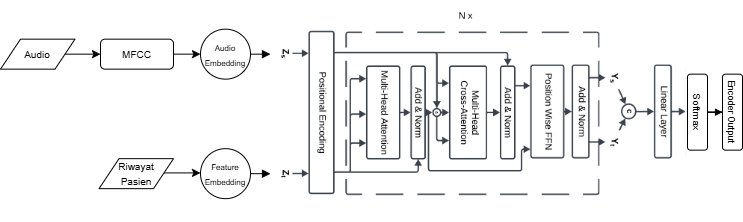
\includegraphics[width=1\linewidth]{gambar/Arsitektur Model.png}
        \caption{Desain rancangan arsitektur model.}
        \label{fig:model}
    \end{figure}
    Input berupa audio dengan fitur MFCC berukuran \(T \times F\) (dengan \(T\) adalah jumlah frame dan \(F\) adalah jumlah koefisien MFCC) dan data riwayat pasien berukuran \(N \times d_{feat}\) (\(N\) adalah jumlah data riwayat, \(d_{feat}\) adalah dimensi fitur) akan diubah menjadi embedding berukuran \(T \times d_{embed}\) dan \(N \times d_{embed}\) melalui \textit{embedding layer}. \textit{Embedding} ini ditambahkan dengan \textit{positional encoding} dan diteruskan ke \textit{encoder} berbasis transformer, di mana mekanisme \textit{self-attention} dan \textit{cross-attention} digunakan untuk menangkap hubungan antar fitur audio serta interaksi antara audio dan riwayat pasien. Setelah melalui \textit{feedforward network} (FFN), hasil akhir \textit{encoder} berupa \textit{embedding multimodal} dikombinasikan dan diproyeksikan menggunakan linear layer, diikuti oleh \textit{softmax} untuk menghasilkan output akhir dari token [cls] berupa representasi yang dapat digunakan untuk klasifikasi.

    \subsection{\textit{Loss Function}}
    Fungsi kerugian yang digunakan \textit{Categorical Cross-Entropy} untuk setiap kelas \ref{eq:cross_entropy}:
    \begin{equation}
        L(y, \hat{y}) = -\sum_{i=1}^{C} y_i \log(\hat{y}_i)
    \label{eq:cross_entropy}
    \end{equation}
    Keterangan:
    \begin{itemize}
        \item $L(y, \hat{y})$ adalah nilai \textit{Categorical Cross-Entropy}
        \item $y$ adalah nilai target asli
        \item $\hat{y}_i$ adalah nilai prediksi
    \end{itemize}
    
    Di mana $L(y, \hat{y})$ merupakan \textit{categorical cross-entropy loss}. $y_i$ adalah label sebenarnya (0 atau 1 untuk setiap kelas) dari \textit{one-hot encoding} vektor target. $\hat{y}_i$ adalah probabilitas yang diprediksi untuk kelas $i$. $C$ merupakan jumlah kelas yang diprediksi.

    \subsection{Pelatihan Model}
    Penelitian ini akan menggunakan \textit{optimizer} sama dengan yang digunakan Vaswani et al., yaitu \textit{optimizer} Adam \cite{ahn2024understandingadamoptimizeronline} yang menggabungkan momentum dengan RMSprop. Model akan dilatih menggunakan \textit{Notebook Kaggle} dengan GPU NVIDIA Tesla P100-PCIE-16GB untuk model \textit{small} dan \textit{big}. Beberapa kedalaman \textit{layer} dan jumlah \textit{head attention} akan diuji performanya dengan tetap memperhatikan batasan komputasi.
\begin{algorithm}[H]
    \caption{Pelatihan Model}
    \begin{algorithmic}[1]
        \State \textbf{Inisialisasi:} $m_0 \gets 0, v_0 \gets 0, t \gets 0, \beta_1 \gets 0.9, \beta_2 \gets 0.98, \epsilon \gets 10^{-9}$
        \State \textbf{Inisialisasi:} epochs, batch\_size
        \While{epoch $\to$ epochs}
            \While{step $\to$ N // batch\_size}
                \State $lr \gets (d_{embed}^{-0.5} \cdot min(step^{-0.5}, \, step \times    4000^{-1.5}))$
                \State $t \gets t + 1$
                
                \State $g_t \gets \nabla_\theta \mathcal{L}(\theta_{t-1}) \quad \text{(Gradien  \textit{loss function})}$
                
                \State $m_t \gets \beta_1 \cdot m_{t-1} + (1 - \beta_1) \cdot g_t \quad     \text{(Update momentum pertama)}$
                
                \State $v_t \gets \beta_2 \cdot v_{t-1} + (1 - \beta_2) \cdot g_t^2 \quad   \text{(Update momentum kedua)}$
                
                \State $\hat{m}_t \gets m_t / (1 - \beta_1^t) \quad \text{(Koreksi bias     momentum pertama)}$
    
                \State $\hat{v}_t \gets v_t / (1 - \beta_2^t) \quad \text{(Koreksi bias     momentum kedua)}$
    
                \State $\theta_{t} \gets \theta_{t-1} - lr \cdot \hat{m}_t / (\sqrt{\hat{v}_t +     \epsilon}) \quad \text{(Update parameter)}$
            \EndWhile
        \EndWhile
        \State \textbf{\textit{Return}:} Parameter $\theta_t$
    \end{algorithmic}
\end{algorithm}


\section{Evaluasi Model}
	\subsection{\textit{Confusion Matrix}}
    \textit{Confussion matrix} adalah metode dalam pembelajaran mesin yang menyediakan representasi visual dari performa model dalam tugas klasifikasi \cite{10708595}. Matriks ini merangkum prediksi yang benar dan salah yang dibuat oleh model, yang memungkinkan penghitungan berbagai metrik kinerja seperti akurasi, presisi, \textit{recall}, dan \textit{F1-score}. Matriks ini biasanya terdiri dari empat komponen: \textit{True Positive}, \textit{True Negarive}, \textit{False Positive}, dan \textit{False Negative} \ref{tab:confusion_matrix_and_metrics}.
    
    \begin{table}[h]
        \centering
        \caption{\textit{Confusion Matrix} untuk 3 Kelas (a), Rumus metrik evaluasi (b)}
        \begin{minipage}{0.5\textwidth}
          \centering
          \begin{tabular}{c c c c c}
            \hline
            \multicolumn{2}{c}{\textbf{Actual Class}} & \multicolumn{3}{c}{\textbf{Predicted Class}} \\
            \hline
            \multicolumn{2}{c}{} & \cellcolor{gray!20}$C_1$ & \cellcolor{gray!20}$C_2$ &    \cellcolor{gray!20}$C_3$ \\
            \multirow{3}{*}{\rotatebox{90}{\textbf{Actual}}} 
            & \cellcolor{gray!20}$C_1$ & \cellcolor{green!20}TP$_{1}$ & FP$_{12}$ & FP$_{13}$ \\
            
            & \cellcolor{gray!20}$C_2$ & FN$_{21}$ & \cellcolor{green!20}TP$_{2}$ & FP$_{23}$ \\
            
            & \cellcolor{gray!20}$C_3$ & FN$_{31}$ & FN$_{32}$ & \cellcolor{green!20}TP$_{3}$ \\
            \hline
          \end{tabular}
          \subcaption{}
        \end{minipage}%
        \begin{minipage}{0.5\textwidth}
          \centering
          \begin{tabular}{l l}
          \hline
          \textbf{Metrik} & \textbf{Rumus} \\
          \hline\\
          Accuracy & $\frac{TP + TN}{TP + TN + FP + FN}$ \\
          \\
          Precision & $\frac{TP}{TP + FP}$ \\
          \\
          Recall & $\frac{TP}{TP + FN}$ \\
          \\
          F1-Score & $2 \times \frac{\text{Precision} \times \text{Recall}}{\text{Precision} +  \text{Recall}}$ \\\\
          \hline
          \end{tabular}
          \subcaption{}
        \end{minipage}
        \label{tab:confusion_matrix_and_metrics}
    \end{table}
    
    \subsection{Kurva ROC-AUC}
    Kurva ROC-AUC merupakan metode untuk mengevaluasi keakuratan algoritma klasifikasi, yang memberikan wawasan tentang kinerjanya di berbagai ambang batas. Kurva ini mengukur keseimbangan antara sensitivitas (\textit{true positive rate}) dan spesifisitas (\textit{false positive rate}), yang memungkinkan penilaian komprehensif terhadap efektivitas model \cite{10420319}.
    % Requires: \usepackage{amsmath}
\begin{equation}
   \text{TPR/sensitivitas} = \frac{\text{TP}}{\text{TP} + \text{FN}}
   \label{eq:tpr}
\end{equation}
\begin{equation}
   \text{FPR/spesifisitas} = \frac{\text{FP}}{\text{FP} + \text{TN}}
   \label{eq:fpr}
\end{equation}
\begin{figure}[H]
    \centering
    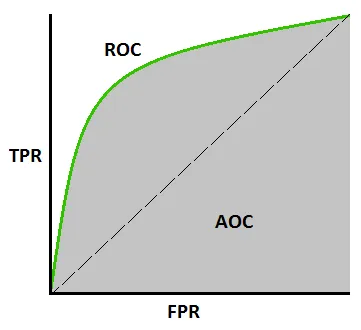
\includegraphics[width=0.4\linewidth]{gambar/ROC-AUC.png}
    \caption{Kurva ROC-AUC}
    \label{fig:roc_auc}
\end{figure}
% Baris ini digunakan untuk membantu dalam melakukan sitasi
% Karena diapit dengan comment, maka baris ini akan diabaikan
% oleh compiler LaTeX.
\begin{comment}
\bibliography{daftar-pustaka}
\end{comment}
